\chapter{TINJAUAN PUSTAKA}

% Ubah konten-konten berikut sesuai dengan isi dari tinjauan pustaka
\section{Hasil penelitian/perancangan terdahulu}

Pada penelitian yang berjudul "\emph{Task-Level Intelligent Human-Robot Interaction
for Assisting Multi-objective Autonomous Grasping Decision with Quadruped Robots}"
\parencite{QifanZhang_tlihrifamoagdwqr}, Zhang et al. mengusulkan pendekatan
interaksi manusia-robot (HRI) berbasis \emph{task-level} untuk meningkatkan kemampuan robot \emph{quadruped}
dalam mengambil keputusan saat melakukan \emph{grasping} terhadap beberapa objek secara otonom.
Dalam penelitian ini, sistem yang dikembangkan bertujuan untuk mengatasi keterbatasan sistem
\emph{grasping} otonom pada robot \emph{quadruped} yang umumnya memiliki kapabilitas pengambilan keputusan
yang terbatas serta minim interaksi dengan operator manusia. Penelitian ini merancang sebuah terminal kontrol
yang dilengkapi dengan layar sentuh, memungkinkan operator untuk secara intuitif menentukan
pusat pencarian objek melalui tampilan video yang diterima dari robot.
Eksperimen yang dilakukan dalam lingkungan nyata menunjukkan bahwa metode ini efektif dalam
menangani skenario \emph{multi-target} \emph{grasping} dan meningkatkan pengambilan keputusan robot \emph{quadruped}
saat menghadapi berbagai objek.

Dalam penelitian lain yang berjudul "\emph{Scene Prediction and Manipulator Grasp Pose
Estimation Based on YOLO-GraspNet}"\parencite{LiWanyan_spamgpeboyg}, Wanyan et al. mengusulkan
algoritma estimasi posisi berbasis prediksi skenario yang disebut YOLO-GraspNet untuk
meningkatkan akurasi dan kecepatan dalam proses \emph{grasping} oleh lengan robot, terutama dalam
menangani objek dengan bentuk tidak beraturan di lingkungan yang kompleks.
Metode yang dikembangkan terdiri dari dua tahap utama. Pada tahap pertama, model YOLOv5s
digunakan untuk mengidentifikasi dan menentukan lokasi target \emph{grasping}, serta menandai informasi
kedalaman dari area target yang telah terdeteksi. Dengan demikian, hanya area yang relevan
yang akan diproses lebih lanjut, sehingga mengurangi jumlah data yang perlu diproses dan
meningkatkan efisiensi sistem. Selanjutnya, pada tahap kedua, jaringan GraspNet digunakan
untuk memproses data dari area yang telah ditandai guna memperkirakan \emph{pose} \emph{grasping} yang optimal.
Dengan mengombinasikan keunggulan YOLOv5s dalam deteksi objek yang cepat dan akurat serta
kemampuan GraspNet dalam prediksi \emph{pose} \emph{grasping} yang presisi, metode ini dapat mengatasi
tantangan utama yang dihadapi oleh pendekatan konvensional, seperti jumlah data masukan yang besar,
kecepatan perhitungan yang lambat, dan ketidakakuratan dalam menentukan posisi objek dengan bentuk kompleks.

% Terminal kontrol menerima umpan video langsung dari robot melalui pemancar video, kemudian menampilkan gambar yang telah
% didekodekan dalam antarmuka grafis (GUI). Dengan memilih titik tertentu dalam gambar sebagai pusat
% pencarian, sistem pengenalan target yang diterapkan akan menggunakan prinsip jarak Euclidean terpendek
% untuk mencari objek yang paling relevan dalam area sekitar titik yang dipilih. Setelah
% target grasping ditentukan, sistem kemudian secara otomatis memulai perencanaan lintasan
% serta deteksi grasping untuk mengeksekusi tugas manipulasi objek. 

\section{Teori/Konsep Dasar}

% \subsection{Hukum Newton}

% % Contoh penggunaan referensi dari pustaka
% Newton pernah merumuskan \parencite{Newton1687} bahwa \lipsum[8]
% % Contoh penggunaan referensi dari persamaan
% Kemudian menjadi persamaan seperti pada persamaan \ref{eq:FirstLaw}.
% % Contoh pembuatan persamaan
% \begin{equation}
%   % Label referensi dari persamaan yang dibuat
%   \label{eq:FirstLaw}
%   % Baris kode persamaan yang dibuat
%   \sum \mathbf{F} = 0\; \Leftrightarrow\; \frac{\mathrm{d} \mathbf{v} }{\mathrm{d}t} = 0.
% \end{equation}
% \lipsum[9]

\subsection{Robot \emph{Quadruped}}

Robot \emph{quadruped} adalah jenis robot berkaki empat yang dirancang untuk meniru gerakan hewan berkaki empat,
seperti anjing, kuda, atau harimau. Berbeda dengan robot beroda atau berkaki dua (bipedal),
robot \emph{quadruped} memiliki keunggulan dalam hal stabilitas dan kemampuan bergerak di berbagai medan yang tidak rata\parencite{AshishMajithia_dmcapoqracr}.
Struktur kaki yang dimiliki memungkinkan robot ini untuk mempertahankan keseimbangan bahkan
saat bergerak di permukaan yang kasar, berbatu, atau licin, menjadikannya solusi ideal untuk
berbagai aplikasi di bidang eksplorasi, pencarian dan penyelamatan, serta industri.  

\begin{figure} [H] \centering
  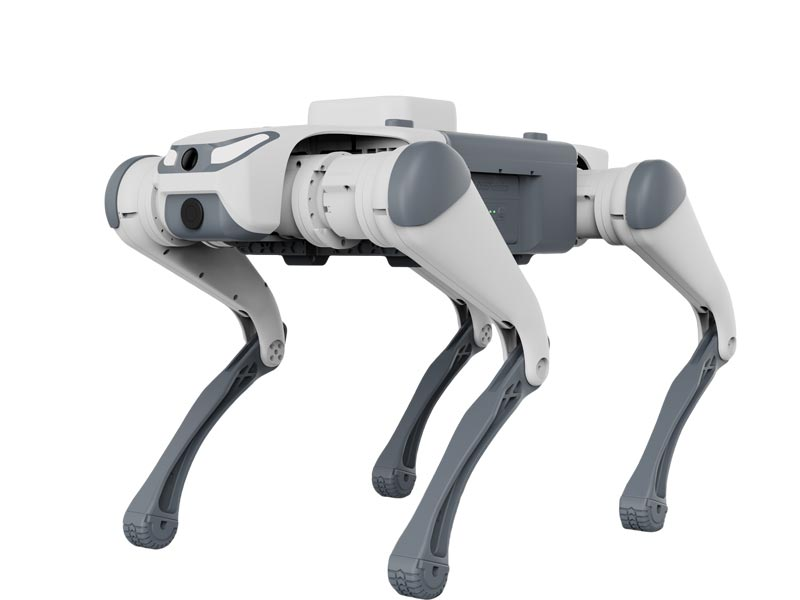
\includegraphics[scale=0.3]{gambar/quadruped_robot.jpg}
  \caption{DeepRobotics Lite3\parencite{img_QuadrupedRobot}}
  \label{fig:quadruped_robot}
\end{figure}

Dalam hal desain dan kontrol, robot \emph{quadruped} mengadopsi prinsip-prinsip biomekanika
untuk meniru pola gerak alami hewan. Pola gerak ini, yang dikenal sebagai \emph{gait},
mencakup berbagai cara berjalan seperti \emph{trot}, \emph{pace}, dan \emph{gallop},
yang masing-masing digunakan tergantung pada kecepatan dan kondisi medan.
Implementasi gerakan ini membutuhkan sistem kendali yang kompleks,
termasuk algoritma keseimbangan dinamis dan kontrol koordinasi antar kaki.
Beberapa robot \emph{quadruped} menggunakan sensor inersia (IMU), kamera,
serta teknologi kecerdasan buatan (AI) untuk meningkatkan kesadaran situasional dan kemampuan navigasi secara otonom.  

Robot \emph{quadruped} dapat dikategorikan berdasarkan sistem aktuasi yang digunakan,
yaitu robot dengan aktuasi elektrik, hidraulik, atau kombinasi keduanya.
Robot dengan aktuator elektrik cenderung lebih ringan dan lebih efisien dalam hal konsumsi daya,
sementara robot hidraulik lebih kuat dan mampu menangani beban yang lebih berat.
Beberapa robot \emph{quadruped} yang telah dikembangkan termasuk Spot dari Boston Dynamics,
ANYmal dari ANYbotics, dan Unitree Go1, yang digunakan dalam berbagai penelitian dan aplikasi industri.  

Penggunaan robot \emph{quadruped} terus berkembang, terutama dalam bidang militer, eksplorasi luar angkasa,
pertanian, dan robotika layanan. Dengan kemampuannya untuk bergerak secara fleksibel di medan yang menantang
dan membawa beban tambahan, robot ini memiliki potensi besar untuk digunakan dalam
skenario di mana robot beroda atau berkaki dua mengalami kesulitan.
Tantangan utama dalam pengembangan robot \emph{quadruped} meliputi efisiensi energi, ketahanan perangkat keras,
dan peningkatan kecerdasan buatan agar mampu beradaptasi lebih baik dengan lingkungan yang tidak terstruktur.

\subsection{Robot Lengan}

\begin{figure} [H] \centering
  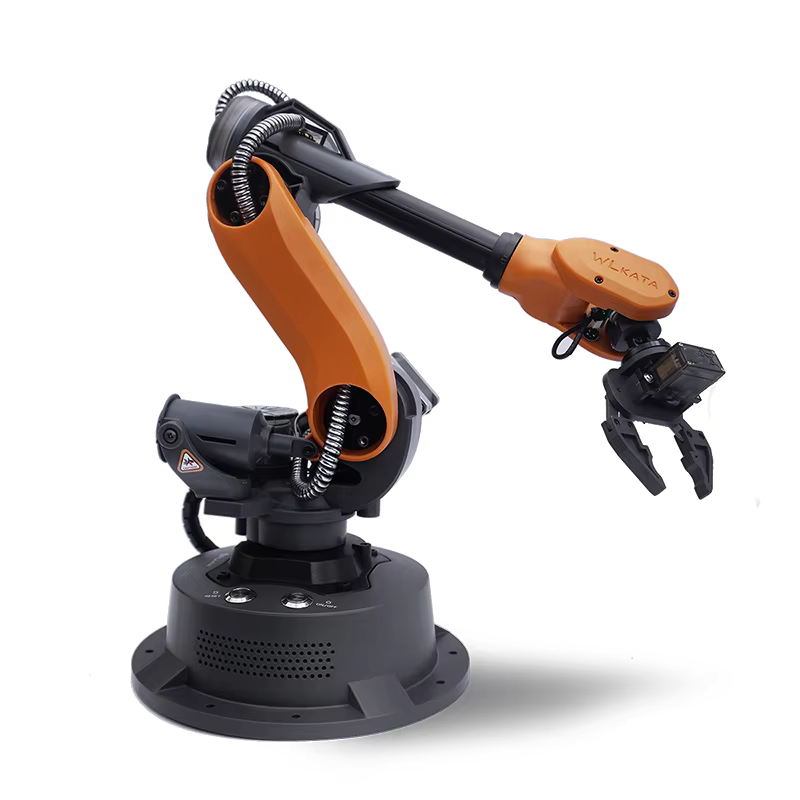
\includegraphics[scale=0.25]{gambar/arm_robot.png}
  \caption{Salah Satu Jenis Robot Lengan Dari Wlkata\parencite{img_ArmRobot}}
  \label{fig:arm_robot}
\end{figure}
Robot lengan, atau \emph{robotic arm}, adalah jenis robot yang dirancang untuk meniru fungsi lengan manusia
dalam melakukan berbagai tugas manipulasi objek. Robot ini umumnya terdiri dari serangkaian sambungan (\emph{joints})
dan batang (\emph{links}) yang memungkinkan pergerakan fleksibel dalam berbagai arah. Dengan kombinasi aktuator,
sensor, dan sistem kendali yang kompleks, robot lengan mampu melakukan tugas-tugas seperti \emph{pick-and-place},
perakitan, pengelasan, pengecatan, serta tugas presisi lainnya dalam industri manufaktur, medis, dan penelitian.

Robot lengan dapat dikategorikan berdasarkan konfigurasi kinematiknya, seperti robot kartesian,
robot SCARA (\emph{Selective Compliance Articulated Robot Arm}), robot artikulasi, dan robot delta.
Robot kartesian memiliki tiga derajat kebebasan dalam sumbu X, Y, dan Z, serta sering digunakan
dalam aplikasi yang membutuhkan pergerakan linier, seperti mesin CNC. Robot SCARA memiliki fleksibilitas
lebih dalam bidang horizontal dan umumnya digunakan dalam proses perakitan cepat. Robot artikulasi,
yang memiliki sambungan berputar serupa dengan lengan manusia, digunakan dalam berbagai aplikasi industri
dan medis karena kemampuannya untuk mencapai berbagai sudut dan melakukan gerakan yang kompleks.
Sementara itu, robot delta, yang memiliki struktur paralel, biasanya diterapkan dalam industri makanan
dan farmasi untuk tugas-tugas kecepatan tinggi dengan presisi tinggi.

Dalam implementasi teknologinya, robot lengan menggunakan berbagai sensor dan aktuator untuk
meningkatkan akurasi dan efisiensi operasional\parencite{ZhenXie_lbrgar}. Sensor posisi dan kecepatan digunakan untuk
mengontrol gerakan sendi, sementara sensor gaya dan torsi memungkinkan robot berinteraksi
dengan lingkungan secara lebih presisi, misalnya dalam tugas perakitan yang membutuhkan kepekaan
terhadap perubahan gaya. Kamera dan sistem visi komputer juga sering digunakan untuk mendeteksi
dan mengenali objek, memungkinkan robot melakukan tugas-tugas berbasis kecerdasan buatan
seperti penyortiran otomatis dan inspeksi kualitas produk.

Sistem kendali robot lengan dapat dibagi menjadi kontrol terbuka (\emph{open-loop control}) dan
kontrol tertutup (\emph{closed-loop control}). Dalam sistem kontrol terbuka, perintah gerakan diberikan
tanpa umpan balik dari sensor, sementara dalam kontrol tertutup, sistem terus memantau dan
menyesuaikan gerakan berdasarkan informasi dari sensor, sehingga menghasilkan pergerakan
yang lebih akurat dan adaptif. Algoritma kendali seperti \emph{PID control}, \emph{inverse kinematics},
dan \emph{reinforcement learning} sering digunakan untuk meningkatkan performa robot dalam
menyesuaikan gerakan terhadap tugas tertentu.

Robot lengan telah menjadi bagian penting dalam revolusi industri dan otomatisasi modern.
Dalam industri manufaktur, robot ini digunakan untuk meningkatkan produktivitas dan
mengurangi risiko cedera pada pekerja manusia. Di bidang medis, robot bedah seperti
da Vinci Surgical System memungkinkan prosedur bedah yang lebih presisi dan minim invasif.
Selain itu, dalam dunia penelitian dan eksplorasi luar angkasa, robot lengan digunakan
dalam eksperimen ilmiah dan misi eksplorasi, seperti lengan robotik yang dipasang pada \emph{rover} penjelajah Mars.

\subsection{Human-Robot Interaction}

\subsection{Grasping Pose Detection}

\subsection{Pengolahan Citra}

\subsection{ROS}

\subsection{GraspNet}